\documentclass[conference]{IEEEtran}
\usepackage[utf8]{inputenc}
\usepackage{cite}
\usepackage{tabularx} % Required for the table
\usepackage{array}    % Required for custom column types
\usepackage{longtable}
\usepackage{booktabs}
\usepackage{adjustbox} % To allow scaling of tables
\usepackage{caption}
\usepackage{stfloats}
\usepackage{authblk}
\usepackage{algorithm}      % For algorithm environment
\usepackage{algpseudocode}  % For algorithmicx commands
\usepackage{amsmath}
\usepackage{float}
\usepackage{amsmath}
\usepackage{graphicx}
\usepackage{subcaption}  % This is the correct package

\begin{document}
	
	\title{Power, Area and Thermal Prediction in 3D Network-on-Chip using Machine Learning}
	
	\author{Abhijith C, Anand M K \\
		
		Department of Computer Science and Engineering \\ 
		National Institute of Technology Karnataka (NITK) \\ 
		Surathkal, India\\
		Email: \{abhijithc.242cs003, anandmk.242cs008\}@nitk.edu.in}
	
	
	\maketitle
	
\section{Experimental Results}
This section focuses on the experimental setup, dataset generation, dataset preprocessing, performance of different models, and comparison of their performance.

	\subsection{Experimental Setup}
	The dataset is generated using PAT-Noxim and a shell script.PAT Noxim is a cycle-accurate simulator used to analyze power, area, and thermal metrics in networks-on-chip (NoC) architectures. The entire experiment is executed on a computer setup with the configurations: HP HP EliteDesk 800 G8 Tower PC, 16.0 GiB memory, 11th Gen Intel® Core™ i5-11500 @ 2.70GHz × 12 graphics, Mesa Intel® Graphics (RKL GT1), 1.0 TB disk capacity and Ubuntu 22.04.4 LTS.
	
	\subsection{Dataset Generation}
	The parameters used in NoC architecture configuration are as follows.
	\begin{itemize}
		\item \textbf{dimx/ dimy/ dimz}: Represents the dimensions of the NoC architecture in X, Y, and Z directions.
		\item \textbf{PIR (Packet Injection Rate)}: The rate at which packets are injected into the network.
		\item \textbf{Buffer Size}: Storage capacity of the input buffers in each router.
		\item \textbf{Routing Type}: Represents the packet routing algorithms, such as XYZ routing, OE 3D, or Fully adaptive routing.
		\begin{itemize}
			\item \textbf{XYZ (XYZ Routing)}:  Packets are routed in three dimensions sequentially.
			\item \textbf{OE3D (Odd-Even 3D Routing)}: Extends the 2D odd-even routing strategy to three dimensions.
			\item \textbf{Fully Adaptive Routing}: The path of each packet is determined based on congestion and link availability.
		\end{itemize}
		\item \textbf{Traffic Type}: Represents the data traffic pattern in the network, such as Random.
		\begin{itemize}
			\item \textbf{Random Traffic}: The source-destination pairs for packet communication are selected randomly.
		\end{itemize}
		\item \textbf{Cycles}: Represents the number of simulation cycles the simulator runs.
		
	\end{itemize}
	The dataset is generated by simulating various configurations on PAT-Noxim. The configurations include mesh sizes ranging from 2 x 2 x 2 to  16 x 16 x 2, pir values from 0.01 to 0.1 with step size of 0.01, and buffer sizes 4, 6, 8, and 10. Three different routing algorithms are used: XYZ, Fully Adaptive, and Odd-Even 3D. The simulations are run for 200000 cycles. The traffic considered is Random. \\
	The simulation output of PAT Noxim consists of the following parameters:
	\begin{itemize}
		\item \textbf{Steady State Temperature}: Refers to the final, stabilized temperature reached by the NoC system.
		\item \textbf{Core Average Temperature}: Represents the average temperature of all the processing cores in the NoC.
		\item \textbf{Memory Average Temperature}: Represents the average temperature of the memory units integrated within the NoC.
		\item \textbf{Router Average Temperature}: Represents the average temperature of all routers in the NoC.
		\item \textbf{Average Power}: Represents the total average power consumption of the NoC system.
		\item \textbf{Average Core Power}: Represents the average power consumption of all cores in the NoC.
		\item \textbf{Average Router Power}: Represents the average power consumption of the routers in the NoC.
		\item \textbf{Average Power Per Router}: Refers to the average power consumption per router in the NoC.
		\item \textbf{Layer Area}: Refers to the area occupied by a single layer in a 3D NoC.
		\item \textbf{Total Area}:  The overall area used by the entire NoC system.
		\item \textbf{Area Per Core}: Refers to the area of each individual core in the NoC system.
	\end{itemize} 

	\subsection{Data Preprocessing}
	The simulation results of PAT-Noxim include various metrics. The parameters considered in this experiment are power metrics such as average power, average core power, average router power, and average power per router; area metrics such as layer area, area per core, and total area; temperature metrics such as steady state temperature, core average temperature, memory average temperature, and router average temperature. The categorical column, such as the routing algorithm, is encoded. The dataset is split into training and test sets (80\% train and 20\% test). The parameters are standardized to the same scale, which improves the performance of ML models.

	\subsection{Experiments conducted}
	The generated dataset is trained using AdaBoost with Decision Tree as the model. Decision tree regressor is used as a weak learner for the AdaBoost technique. Decision trees are non-linear models that split data based on feature values to predict a target. They are effective for modeling complex relationships between NoC parameters, which makes them ideal for use as base learners for AdaBoost. AdaBoost is an ensemble technique. It assigns weight to misclassified data points so subsequent learners focus on these more complex examples, thus improving accuracy. \\
	The performance of the AdaBoost with decision tree model is then evaluated against a few other models that are trained on the same dataset. The models used are:
	\begin{itemize}
		\item Random Forest
		\item Decision Tree
		\item AdaBoost
		\item Support Vector Regressor (SVR)
		\item Linear Regression
		\item K-Nearest Neighbors
		\item 9-Layer CNN
		\item RNN (LSTM)
		\item Feedforward Neural Network(FNN)
	\end{itemize}
	

	\subsection{Performance Metrics}
	The performance metrics used for evaluating the performance of different models are:	
	\begin{itemize}
		\item \textbf{Mean Squared Error (MSE)}: Measures the average squared difference between the predicted values (\( \hat{y}_i \)) and actual values (\( y_i \)).
		\[
		\text{MSE} = \frac{1}{n} \sum_{i=1}^n \left( y_i - \hat{y}_i \right)^2
		\]
		
		\item \textbf{Mean Absolute Error (MAE)}: Measures the average of the absolute differences between the predicted values (\( \hat{y}_i \)) and actual values (\( y_i \)).
		\[
		\text{MAE} = \frac{1}{n} \sum_{i=1}^n \left| y_i - \hat{y}_i \right|
		\]
		
		\item \textbf{R² (Coefficient of Determination)}: Represents the proportion of variance in the dependent variable (\( y_i \)) explained by the independent variables, where \( \bar{y} \) is the mean of the actual values.
		\[
		R^2 = 1 - \frac{\sum_{i=1}^n \left( y_i - \hat{y}_i \right)^2}{\sum_{i=1}^n \left( y_i - \bar{y} \right)^2}
		\] 
	\end{itemize} 
	

\subsection{Results Analysis}

	\subsubsection{Temperature Analysis}
	This section analyzes temperature-related parameters such as steady-state temperature, core average temperature, memory average temperature, and router average temperature. Tables \ref{tab:steady_state_temp_L0} and \ref{tab:steady_state_temp_L1} analyze layer one and layer two steady-state temperatures. Layer one and two core average temperature metrics are provided in Tables \ref{tab:core_avg_temp_L0} and \ref{tab:core_avg_temp_L1}. Tables \ref{tab:mem_avg_temp_L0} and \ref{tab:mem_avg_temp_L1} analyze layer one and layer two memory average temperatures. Layer one and two router average temperature metrics are provided in Tables \ref{tab:router_avg_temp_L0} and \ref{tab:router_avg_temp_L1}.


\begin{table}[htbp]
	\caption{Performance Metrics for Different Algorithms - steady\_state\_temp\_L0}
	\label{tab:steady_state_temp_L0}
	\begin{tabular}{lccc}
		\toprule
		\textbf{Algorithm} & \textbf{MSE} & \textbf{MAE} & \textbf{\(R^2\)} \\
		\midrule
		AdaBoost with Decision Tree & 0.0011 & 0.0125 & 0.9989 \\
		Random Forest & 0.0012 & 0.0154 & 0.9987 \\
		Decision Tree & 0.0021 & 0.0171 & 0.9978 \\
		KNN & 0.0380 & 0.1171 & 0.9604 \\
		SVR & 0.0613 & 0.1250 & 0.9362 \\
		AdaBoost & 0.1979 & 0.3712 & 0.7939 \\
		Linear Regression & 0.4100 & 0.4848 & 0.5731 \\
		9-Layer CNN        & 0.0252       & 0.0975       & 0.9737      \\ 
		RNN (LSTM)  & 0.0181       & 0.0813       & 0.9812      \\ 
		FNN                & 0.0360       & 0.1298       & 0.9635      \\ 
		\bottomrule
	\end{tabular}
\end{table}


\begin{table}[htbp]
	\caption{Performance Metrics for Different Algorithms - steady\_state\_temp\_L1}
	\label{tab:steady_state_temp_L1}
	\begin{tabular}{lccc}
		\toprule
		\textbf{Algorithm} & \textbf{MSE} & \textbf{MAE} & \textbf{\(R^2\)} \\
		\midrule
		AdaBoost with Decision Tree & 0.0011 & 0.0127 & 0.9988 \\
		Random Forest & 0.0012 & 0.0153 & 0.9987 \\
		Decision Tree & 0.0020 & 0.0169 & 0.9979 \\
		KNN & 0.0383 & 0.1175 & 0.9601 \\
		SVR & 0.0622 & 0.1252 & 0.9353 \\
		AdaBoost & 0.1931 & 0.3624 & 0.7990 \\
		Linear Regression & 0.4123 & 0.4862 & 0.5709 \\
		9-Layer CNN                & 0.0254       & 0.0981       & 0.9736      \\ 
		RNN (LSTM)  & 0.0177       & 0.0801       & 0.9816      \\ 
		FNN                & 0.0362       & 0.1301       & 0.9633      \\ 
		\bottomrule
	\end{tabular}
\end{table}


\begin{table}[htbp]
	\caption{Performance Metrics for Different Algorithms - core\_avg\_temp\_L0}
	\label{tab:core_avg_temp_L0}
	\begin{tabular}{lccc}
		\toprule
		\textbf{Algorithm} & \textbf{MSE} & \textbf{MAE} & \textbf{\(R^2\)} \\
		\midrule
		AdaBoost with Decision Tree & 0.0077 & 0.0415 & 0.9922 \\
		Random Forest & 0.0069 & 0.0436 & 0.9930 \\
		Decision Tree & 0.0106 & 0.0506 & 0.9892 \\
		AdaBoost & 0.3740 & 0.4481 & 0.6203 \\
		KNN & 0.2283 & 0.2017 & 0.7683 \\
		SVR & 0.4741 & 0.2536 & 0.5188 \\
		Linear Regression & 0.6070 & 0.4970 & 0.3839 \\
		9-Layer CNN                & 0.0276       & 0.1096       & 0.9720      \\ 
		RNN (LSTM)  & 0.0398       & 0.1269       & 0.9596      \\ 
		FNN                & 0.0378       & 0.1323       & 0.9627      \\ 
		\bottomrule
	\end{tabular}
\end{table}

\begin{table}[htbp]
	\caption{Performance Metrics for Different Algorithms - core\_avg\_temp\_L1}
	\label{tab:core_avg_temp_L1}
	\begin{tabular}{lccc}
		\toprule
		\textbf{Algorithm} & \textbf{MSE} & \textbf{MAE} & \textbf{\(R^2\)} \\
		\midrule
		AdaBoost with Decision Tree & 0.0034 & 0.0267 & 0.9966 \\
		Random Forest & 0.0027 & 0.0265 & 0.9973 \\
		Decision Tree & 0.0043 & 0.0307 & 0.9958 \\
		SVR & 0.3460 & 0.2720 & 0.6582 \\
		KNN & 0.2191 & 0.2000 & 0.7835 \\
		AdaBoost & 0.2557 & 0.4098 & 0.7474 \\
		Linear Regression & 0.9037 & 0.5865 & 0.1072 \\
		9-Layer CNN                & 0.0213       & 0.0898       & 0.9790      \\ 
		RNN (LSTM)  & 0.0229       & 0.0896       & 0.9774      \\ 
		FNN                & 0.0310       & 0.1200       & 0.9696      \\ 
		\bottomrule
	\end{tabular}
\end{table}
\begin{table}[htbp]
	\caption{Performance Metrics for Different Algorithms - mem\_avg\_temp\_L0}
	\label{tab:mem_avg_temp_L0}
	\begin{tabular}{lccc}
		\toprule
		\textbf{Algorithm} & \textbf{MSE} & \textbf{MAE} & \textbf{\(R^2\)} \\
		\midrule
		AdaBoost with Decision Tree & 0.0064 & 0.0432 & 0.9936 \\
		Random Forest & 0.0051 & 0.0398 & 0.9949 \\
		Decision Tree & 0.0082 & 0.0471 & 0.9918 \\
		KNN & 0.4311 & 0.2576 & 0.5710 \\
		AdaBoost & 0.1985 & 0.3481 & 0.8025 \\
		SVR & 0.9742 & 0.3193 & 0.0304 \\
		Linear Regression & 0.8829 & 0.4742 & 0.1213 \\
		9-Layer CNN                & 0.0349       & 0.1198       & 0.9653      \\ 
		RNN (LSTM)  & 0.0323       & 0.1170       & 0.9679      \\ 
		FNN                & 0.0510       & 0.1589       & 0.9511      \\ 
		\bottomrule
	\end{tabular}
\end{table}
\begin{table}[htbp]
	\caption{Performance Metrics for Different Algorithms - mem\_avg\_temp\_L1}
	\label{tab:mem_avg_temp_L1}
	\begin{tabular}{lccc}
		\toprule
		\textbf{Algorithm} & \textbf{MSE} & \textbf{MAE} & \textbf{\(R^2\)} \\
		\midrule
		AdaBoost with Decision Tree & 0.0020 & 0.0212 & 0.9980 \\
		Random Forest & 0.0017 & 0.0198 & 0.9983 \\
		Decision Tree & 0.0030 & 0.0235 & 0.9971 \\
		KNN & 0.2512 & 0.2029 & 0.7556 \\
		AdaBoost & 0.1464 & 0.2762 & 0.8576 \\
		SVR & 0.3990 & 0.2770 & 0.6118 \\
		Linear Regression & 1.0030 & 0.5763 & 0.0242 \\
		9-Layer CNN                & 0.0195       & 0.0804       & 0.9810      \\ 
		RNN (LSTM)  & 0.0166       & 0.0774       & 0.9838      \\ 
		FNN                & 0.0314       & 0.1182       & 0.9695      \\ 
		\bottomrule
	\end{tabular}
\end{table}

\begin{table}[htbp]
	\caption{Performance Metrics for Different Algorithms - router\_avg\_temp\_L0}
	\label{tab:router_avg_temp_L0}
	\begin{tabular}{lccc}
		\toprule
		\textbf{Algorithm} & \textbf{MSE} & \textbf{MAE} & \textbf{\(R^2\)} \\
		\midrule
		AdaBoost with Decision Tree & 0.0047 & 0.0313 & 0.9952 \\
		Random Forest & 0.0050 & 0.0362 & 0.9950 \\
		Decision Tree & 0.0075 & 0.0413 & 0.9925 \\
		KNN & 0.2341 & 0.1797 & 0.7651 \\
		AdaBoost & 0.2079 & 0.3494 & 0.7915 \\
		SVR & 0.5236 & 0.2204 & 0.4748 \\
		Linear Regression & 0.5870 & 0.4415 & 0.4112 \\
		9-Layer CNN                & 0.0233       & 0.0906       & 0.9766      \\ 
		RNN (LSTM)  & 0.0229       & 0.0940       & 0.9770      \\ 
		FNN                & 0.0416       & 0.1258       & 0.9593      \\ 
		\bottomrule
	\end{tabular}
\end{table}


\begin{table}[htbp]
	\caption{Performance Metrics for Different Algorithms - router\_avg\_temp\_L1}
	\label{tab:router_avg_temp_L1}
	\begin{tabular}{lccc}
		\toprule
		\textbf{Algorithm} & \textbf{MSE} & \textbf{MAE} & \textbf{\(R^2\)} \\
		\midrule
		AdaBoost with Decision Tree & 0.0020 & 0.0193 & 0.9981 \\
		Random Forest & 0.0020 & 0.0211 & 0.9981 \\
		Decision Tree & 0.0033 & 0.0244 & 0.9968 \\
		KNN & 0.2300 & 0.1786 & 0.7807 \\
		AdaBoost & 0.1616 & 0.3120 & 0.8459 \\
		SVR & 0.3708 & 0.2496 & 0.6464 \\
		Linear Regression & 0.9080 & 0.5579 & 0.1340 \\
		9-Layer CNN                & 0.0156       & 0.0688       & 0.9851      \\ 
		RNN (LSTM)  & 0.0155       & 0.0653       & 0.9853      \\ 
		FNN                & 0.0379       & 0.0851       & 0.9630      \\ 
		\bottomrule
	\end{tabular}
\end{table}
	
	\subsubsection{Power Analysis}
	This section analyzes power-related parameters such as average power, average core power, average power per router, and average router power. Table \ref{tab:avg_cores_power} analyzes the average core power. Average power metrics are provided in Table \ref{tab:avg_power}. Table \ref{tab:avg_power_per_router} analyzes the average power per router. Average router power metrics are provided in Table \ref{tab:avg_routers_power}.

\begin{table}[htbp]
	\caption{Performance Metrics for Different Algorithms - avg\_cores\_power}
	\label{tab:avg_cores_power}
	\begin{tabular}{lccc}
		\toprule
		\textbf{Algorithm} & \textbf{MSE} & \textbf{MAE} & \textbf{\(R^2\)} \\
		\midrule
		AdaBoost with Decision Tree & 0.0004 & 0.0063 & 0.9996 \\
		Random Forest & 0.0004 & 0.0076 & 0.9996 \\
		Decision Tree & 0.0007 & 0.0081 & 0.9993 \\
		SVR & 0.0027 & 0.0429 & 0.9974 \\
		KNN & 0.0062 & 0.0614 & 0.9939 \\
		AdaBoost & 0.0695 & 0.2264 & 0.9309 \\
		Linear Regression & 0.1159 & 0.2551 & 0.8849 \\
		9-Layer CNN                & 0.0043       & 0.0497       & 0.9958      \\ 
		RNN (LSTM)  & 0.0030       & 0.0390       & 0.9970      \\ 
		FNN                & 0.0004       & 0.0076       & 0.9996      \\ 
		\bottomrule
	\end{tabular}
\end{table}


\begin{table}[htbp]
	\caption{Performance Metrics for Different Algorithms - avg\_power}
	\label{tab:avg_power}
	\begin{tabular}{lccc}
		\toprule
		\textbf{Algorithm} & \textbf{MSE} & \textbf{MAE} & \textbf{\(R^2\)} \\
		\midrule
		AdaBoost with Decision Tree & 0.0007 & 0.0086 & 0.9993 \\
		Random Forest & 0.0007 & 0.0101 & 0.9993 \\
		Decision Tree & 0.0012 & 0.0108 & 0.9988 \\
		SVR & 0.0029 & 0.0427 & 0.9971 \\
		KNN & 0.0066 & 0.0611 & 0.9933 \\
		AdaBoost & 0.1072 & 0.2854 & 0.8927 \\
		Linear Regression & 0.1355 & 0.2651 & 0.8644 \\
		9-Layer CNN                & 0.0045       & 0.0499       & 0.9955      \\ 
		RNN (LSTM)  & 0.0039       & 0.0424       & 0.9961      \\ 
		FNN                & 0.0006       & 0.0096       & 0.9994      \\ 
		\bottomrule
	\end{tabular}
\end{table}

\begin{table}[htbp]
	\caption{Performance Metrics for Different Algorithms - avg\_power\_per\_router}
	\label{tab:avg_power_per_router}
	\begin{tabular}{lccc}
		\toprule
		\textbf{Algorithm} & \textbf{MSE} & \textbf{MAE} & \textbf{\(R^2\)} \\
		\midrule
		AdaBoost with Decision Tree & 0.0040 & 0.0204 & 0.9959 \\
		Random Forest & 0.0079 & 0.0371 & 0.9919 \\
		KNN & 0.0080 & 0.0368 & 0.9918 \\
		Decision Tree & 0.0121 & 0.0393 & 0.9877 \\
		SVR & 0.0143 & 0.0796 & 0.9854 \\
		AdaBoost & 0.1188 & 0.2933 & 0.8785 \\
		Linear Regression & 0.1873 & 0.3189 & 0.8085 \\
		9-Layer CNN                & 0.0139       & 0.0795       & 0.9858      \\ 
		RNN (LSTM)  & 0.0197       & 0.0947       & 0.9799      \\ 
		FNN                & 0.0063       & 0.0337       & 0.9936      \\ 
		\bottomrule
	\end{tabular}
\end{table}

\begin{table}[htbp]
	\caption{Performance Metrics for Different Algorithms - avg\_routers\_power}
	\label{tab:avg_routers_power}
	\begin{tabular}{lccc}
		\toprule
		\textbf{Algorithm} & \textbf{MSE} & \textbf{MAE} & \textbf{\(R^2\)} \\
		\midrule
		AdaBoost with Decision Tree & 0.0012 & 0.0123 & 0.9987 \\
		Random Forest & 0.0023 & 0.0170 & 0.9976 \\
		Decision Tree & 0.0034 & 0.0186 & 0.9965 \\
		SVR & 0.0058 & 0.0494 & 0.9941 \\
		KNN & 0.0085 & 0.0552 & 0.9913 \\
		AdaBoost & 0.2717 & 0.4722 & 0.7219 \\
		Linear Regression & 0.2406 & 0.3368 & 0.7537 \\
		9-Layer CNN                & 0.0066       & 0.0550       & 0.9933      \\ 
		RNN (LSTM)  & 0.0075       & 0.0504       & 0.9923      \\ 
		FNN                & 0.0019       & 0.0159       & 0.9981      \\ 
		\bottomrule
	\end{tabular}
\end{table}



	\subsubsection{Area Analysis}
	This section analyzes area-related parameters such as layer area, total area, and area per core. Table \ref{tab:layer_area} analyzes the layer area. Total area metrics are provided in Table \ref{tab:total_area}. Table \ref{tab:area_per_core} analyzes the area per core.

\begin{table}[htbp]
	\caption{Performance Metrics for Different Algorithms - layer\_area}
	\label{tab:layer_area}
	\begin{tabular}{lccc}
		\toprule
		\textbf{Algorithm} & \textbf{MSE} & \textbf{MAE} & \textbf{\(R^2\)} \\
		\midrule
		AdaBoost with Decision Tree & 2.12E-09 & 2.22E-06 & 0.9999 \\
		Random Forest & 8.04E-05 & 0.0029 & 0.9999 \\
		Decision Tree & 0.0003 & 0.0025 & 0.9997 \\
		SVR & 0.0041 & 0.0568 & 0.9960 \\
		KNN & 0.0057 & 0.0594 & 0.9944 \\
		AdaBoost & 0.0335 & 0.1462 & 0.9673 \\
		Linear Regression & 0.1023 & 0.2403 & 0.9000 \\
		9-Layer CNN                & 0.0042       & 0.0493       & 0.9959      \\ 
		RNN (LSTM)  & 0.0025       & 0.0375       & 0.9976      \\ 
		FNN                & 0.0001       & 0.0036       & 0.9999      \\ 
		\bottomrule
	\end{tabular}
\end{table}

\begin{table}[htbp]
	\caption{Performance Metrics for Different Algorithms - total\_area}
	\label{tab:total_area}
	\begin{tabular}{lccc}
		\toprule
		\textbf{Algorithm} & \textbf{MSE} & \textbf{MAE} & \textbf{\(R^2\)} \\
		\midrule
		AdaBoost with Decision Tree & 1.81E-10 & 6.88E-07 & 0.9999 \\
		Random Forest & 8.04E-05 & 0.0029 & 0.9999 \\
		Decision Tree & 0.0003 & 0.0025 & 0.9997 \\
		SVR & 0.0041 & 0.0568 & 0.9960 \\
		KNN & 0.0057 & 0.0594 & 0.9944 \\
		AdaBoost & 0.0333 & 0.1469 & 0.9674 \\
		Linear Regression & 0.1023 & 0.2403 & 0.9000 \\
		9-Layer CNN                & 0.0043       & 0.0504       & 0.9957      \\ 
		RNN (LSTM)  & 0.0023       & 0.0354       & 0.9977      \\ 
		FNN                & 0.0001       & 0.0036       & 0.9999      \\ 
		\bottomrule
	\end{tabular}
\end{table}

\begin{table}[htbp]

	\caption{Performance Metrics for Different Algorithms - area\_per\_core}
	\label{tab:area_per_core}
	\begin{tabular}{lccc}
		\toprule
		\textbf{Algorithm} & \textbf{MSE} & \textbf{MAE} & \textbf{\(R^2\)} \\
		\midrule
		AdaBoost with Decision Tree & 0 & 0 & 1 \\
		AdaBoost & 0 & 0 & 1 \\
		Random Forest & 0 & 0 & 1 \\
		Decision Tree & 0 & 0 & 1 \\
		SVR & 0 & 0 & 1 \\
		KNN & 0 & 0 & 1 \\
		Linear Regression & 0 & 0 & 1 \\
		9-Layer CNN                & 0       & 0       & 1      \\ 
		RNN (LSTM)  & 0       & 0       & 1      \\ 
		FNN                & 0       & 0       & 1      \\ 
		\bottomrule
	\end{tabular}
\end{table}

\subsection{Comparison study}

	\subsubsection{Temperature Analysis}
	This section compares the performance of different models across parameters such as steady-state temperature, core average temperature, memory average temperature, and router average temperature. After studying Tables \ref{tab:steady_state_temp_L0} and \ref{tab:steady_state_temp_L1}, it is evident that AdaBoost with Decision Tree and Random Forest achieved minimal errors (MSE, MAE) and the highest $R^2$ values ($\geq$0.998 $\geq$0.998) for both layers. Algorithms like KNN and SVR had higher errors and lower $R^2$ values. Tables \ref{tab:core_avg_temp_L0}, \ref{tab:core_avg_temp_L1}, \ref{tab:mem_avg_temp_L0}, \ref{tab:mem_avg_temp_L1}, \ref{tab:router_avg_temp_L0}, and \ref{tab:router_avg_temp_L1} show that AdaBoost with Decision Tree and Random Forest performs well with minimal MSE and MAE values and $R^2$ values close to 1 across both layers. Linear regression and SVR show the worst performance.
	
	\subsubsection{Power Analysis}
	This section compares the performance of different models across parameters such as average power, average core power, average power per router, and average router power. After studying Table \ref{tab:avg_cores_power}, it is evident that AdaBoost with Decision Tree and Random Forest show close to zero errors (MSE, MAE) and the highest $R^2$ values ($\geq$0.99). Algorithms like Linear regression and KNN had higher errors and lower $R^2$ values. Tables \ref{tab:avg_power}, \ref{tab:avg_routers_power}, and \ref{tab:avg_power_per_router} show that AdaBoost with Decision Tree performs better than all other algorithms with minimal MSE and MAE values and $R^2$ values close to 1 for average power metrics. Linear regression and KNN show the worst performance with relatively high errors.
	
	\subsubsection{Area Analysis}
	This section compares the performance of different models across parameters such as layer area, total area, and area per core. After studying Tables \ref{tab:layer_area} and \ref{tab:total_area}, it is evident that AdaBoost with Decision Tree and Random Forest show near-perfect performance with close to zero errors (MSE, MAE) and $R^2$ values close to 1. Algorithms like SVR and KNN had higher errors and lower $R^2$ values. Table \ref{tab:area_per_core} shows that all algorithms made perfect predictions with MSE and MAE values as 0 and $R^2$ value as 1 because the area per core is a constant value.
	
	AdaBoost with Decision Tree and Random Forest consistently outperformed all other models with the lowest MSE and MAE values and the highest $R^2$ values across the prediction of all the power, area, and thermal metrics. Random Forest shows slightly less performance than AdaBoost with Decision Tree. Linear Regression and SVR show the worst performance with higher errors and low $R^2$ values. It is concluded that AdaBoost with Decision Tree is the most consistent and accurate model among all other models. This model works by training a series of 50 decision trees, each aimed at reducing the overall prediction error. Each round assigns higher weights to the samples, which are hard to predict. The subsequent trees give more importance to those challenging cases. The final prediction is the aggregation of each tree, which overall makes a robust prediction model. 

	Figures 1 to 7 compare actual values from PAT Noxim and predicted values from the AdaBoost model with the decision tree. The blue dots are individual data points from the test dataset, where each dot shows how closely the model’s predictions match the actual values. The red dashed line represents the ideal fit where the model’s predictions match the actual values. If points are closely clustered around the red line, this suggests that the model’s predictions are relatively accurate.A larger spread from the red line indicates higher prediction errors. Figures 1 to 4 show that the actual and predicted values are almost identical for the temperature parameters. Temperature is measured in degrees Celsius. The blue points and red lines are nearly perfectly aligned. Figures 5 and 6 illustrate that the predicted and actual values are perfectly aligned, highlighting the effectiveness of the AdaBoost model with the decision tree in predicting power values. Power is calculated in \((\text{J/cycle})\).Figure 7 demonstrates that the area is perfectly predicted by the AdaBoost model with the decision tree. The area is measured in \((\mu\text{m}^2)\).

% Begin the figure environment for two images side by side for each pair of targets
\begin{figure}[htbp]
    % First graph
    \begin{subfigure}{0.24\textwidth}
        \centering
        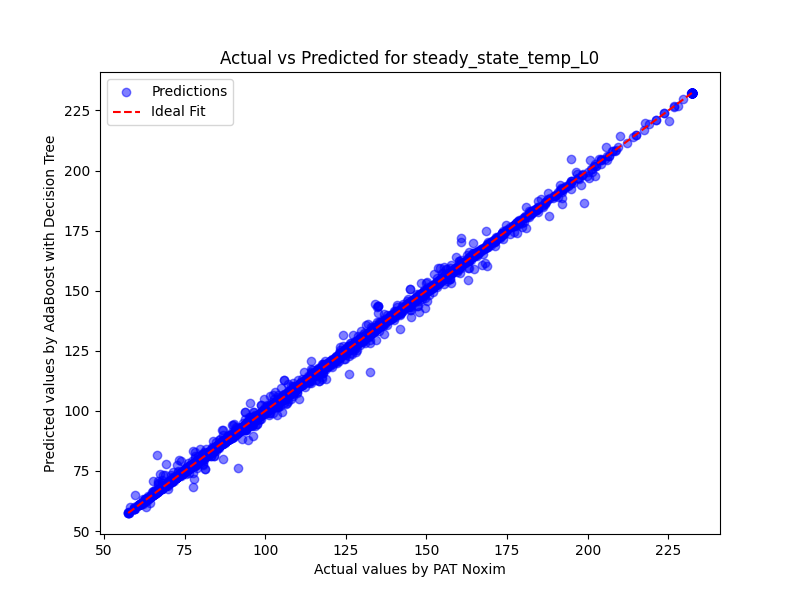
\includegraphics[width=\linewidth]{actual_vs_predicted_steady_state_temp_L0.png}
        \caption{Actual vs Predicted for steady\_state\_temp\_L0}
        \label{fig:actual_vs_predicted_steady_state_temp_L0}
    \end{subfigure}
    \hfill
    % Second graph
    \begin{subfigure}{0.24\textwidth}
        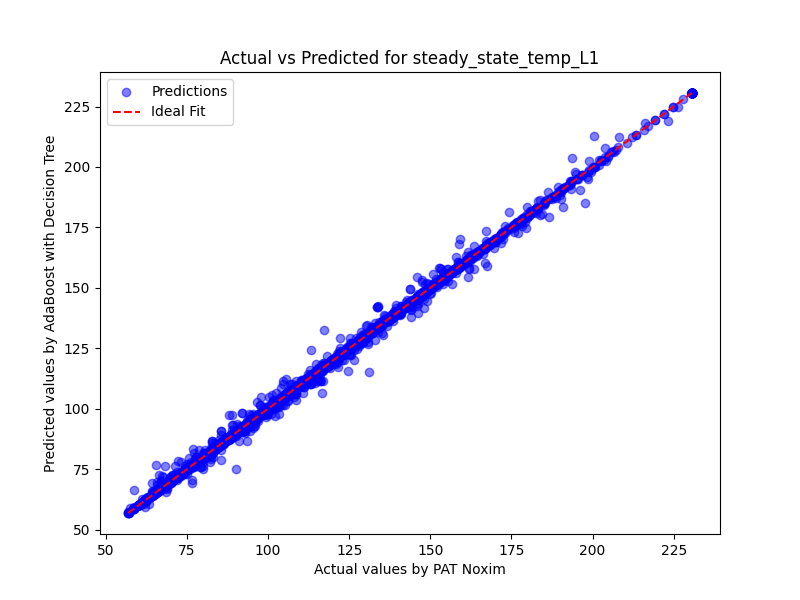
\includegraphics[width=\linewidth]{actual_vs_predicted_steady_state_temp_L1.png}
        \caption{Actual vs Predicted for steady\_state\_temp\_L1}
        \label{fig:actual_vs_predicted_steady_state_temp_L1}
    \end{subfigure}

    \caption{Actual vs Predicted for steady\_state\_temp\_L0 and steady\_state\_temp\_L1}
    \label{fig:side_by_side_graphs_steady_state_temp}
\end{figure}

\begin{figure}[htbp]
    % First graph
    \begin{subfigure}{0.24\textwidth}
        \centering
        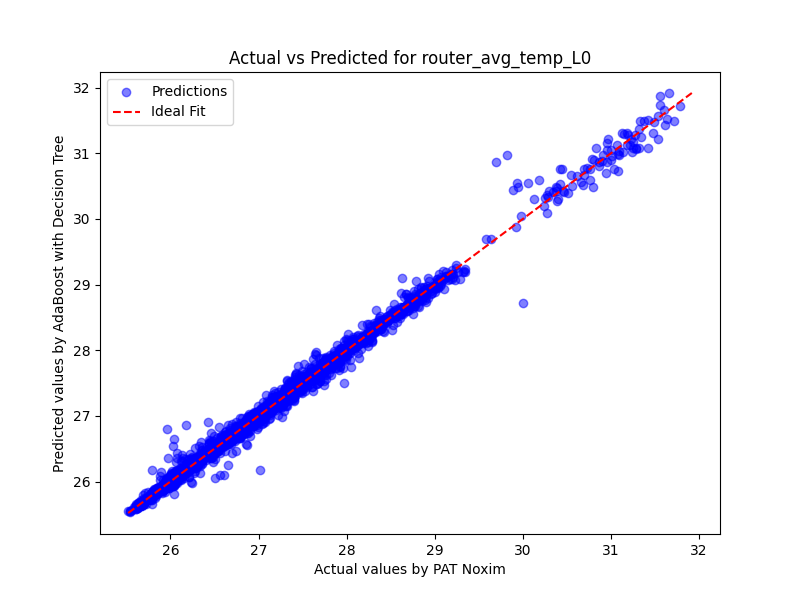
\includegraphics[width=\linewidth]{actual_vs_predicted_router_avg_temp_L0.png}
        \caption{Actual vs Predicted for router\_avg\_temp\_L0}
        \label{fig:actual_vs_predicted_router_avg_temp_L0}
    \end{subfigure}
    \hfill
    % Second graph
    \begin{subfigure}{0.24\textwidth}
        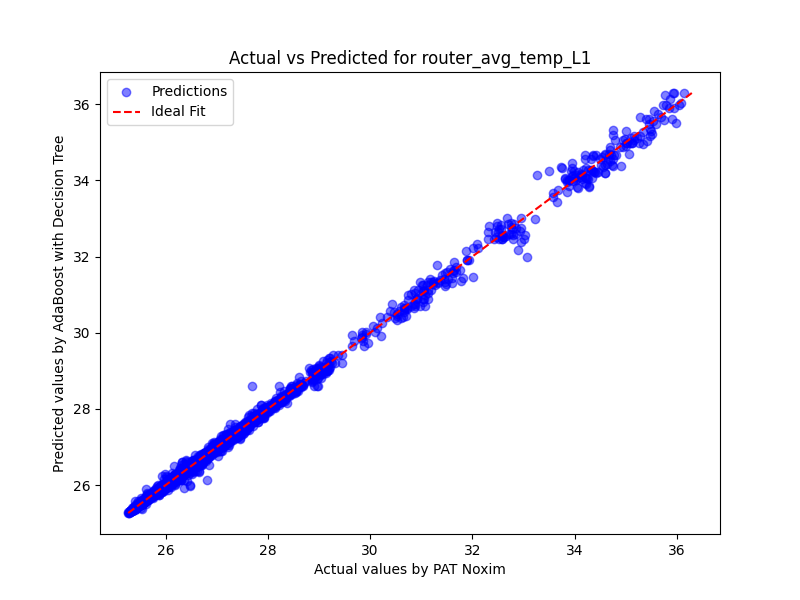
\includegraphics[width=\linewidth]{actual_vs_predicted_router_avg_temp_L1.png}
        \caption{Actual vs Predicted for router\_avg\_temp\_L1}
        \label{fig:actual_vs_predicted_router_avg_temp_L1}
    \end{subfigure}

    \caption{Actual vs Predicted for router\_avg\_temp\_L0 and router\_avg\_temp\_L1}
    \label{fig:side_by_side_graphs_router_avg_temp}
\end{figure}

\begin{figure}[htbp]
    \centering
    % First graph
    \begin{subfigure}{0.24\textwidth}
        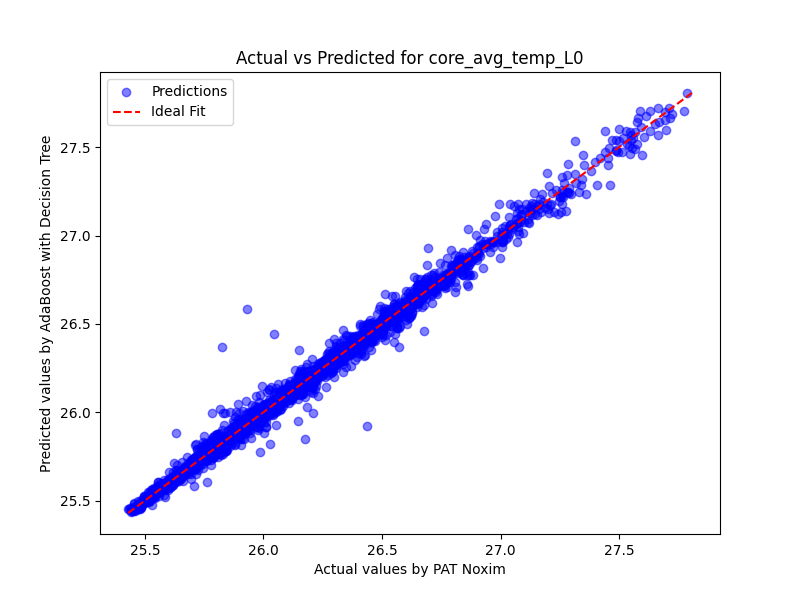
\includegraphics[width=\linewidth]{actual_vs_predicted_core_avg_temp_L0.png}
        \caption{Actual vs Predicted for core\_avg\_temp\_L0}
        \label{fig:actual_vs_predicted_core_avg_temp_L0}
    \end{subfigure}
    \hfill
    % Second graph
    \begin{subfigure}{0.24\textwidth}
        \centering
        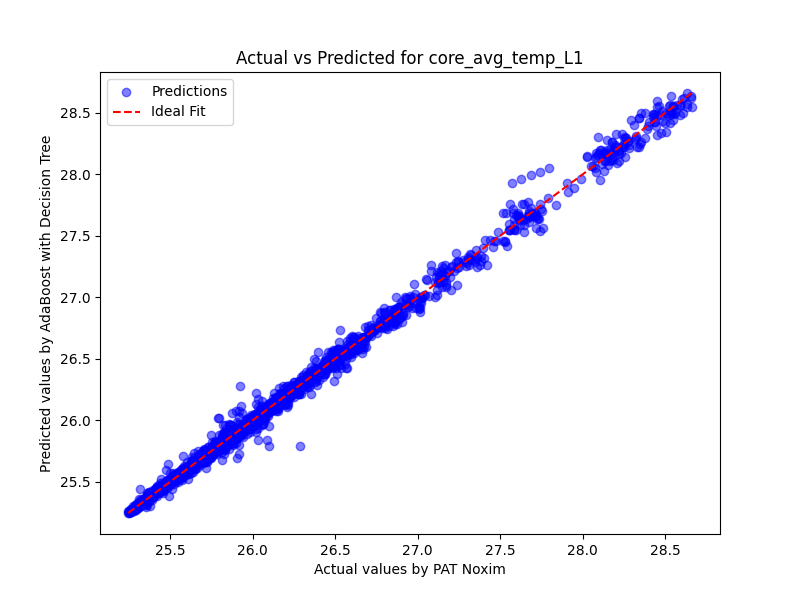
\includegraphics[width=\linewidth]{actual_vs_predicted_core_avg_temp_L1.png}
        \caption{Actual vs Predicted for core\_avg\_temp\_L1}
        \label{fig:actual_vs_predicted_core_avg_temp_L1}
    \end{subfigure}

    \caption{Actual vs Predicted for core\_avg\_temp\_L0 and core\_avg\_temp\_L1}
    \label{fig:side_by_side_graphs_core_avg_temp}
\end{figure}

\begin{figure}[htbp]
    % First graph
    \begin{subfigure}{0.24\textwidth}
        \centering
        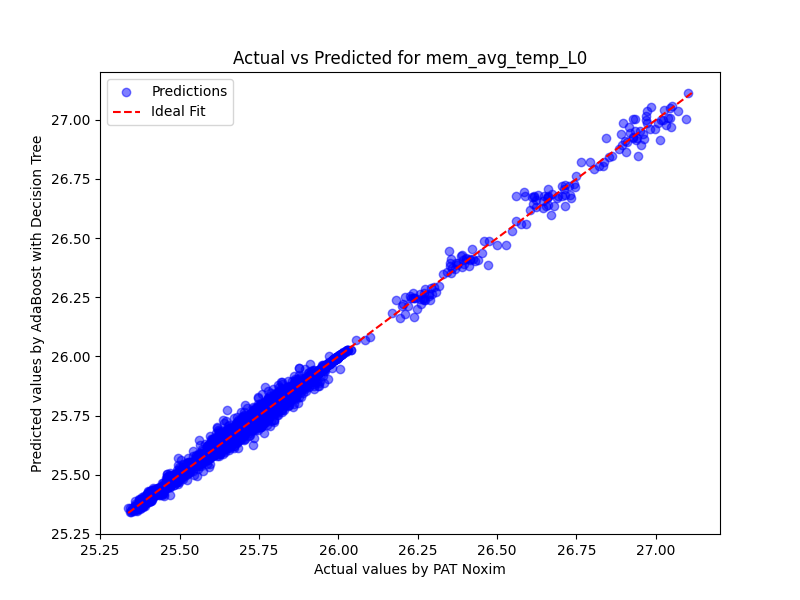
\includegraphics[width=\linewidth]{actual_vs_predicted_mem_avg_temp_L0.png}
        \caption{Actual vs Predicted for mem\_avg\_temp\_L0}
        \label{fig:actual_vs_predicted_mem_avg_temp_L0}
    \end{subfigure}
    \hfill
    % Second graph
    \begin{subfigure}{0.24\textwidth}
        \centering
        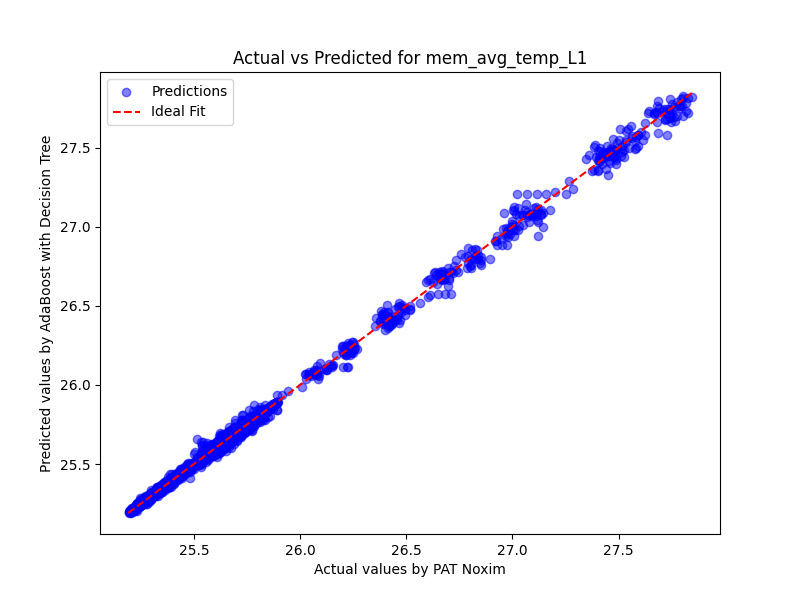
\includegraphics[width=\linewidth]{actual_vs_predicted_mem_avg_temp_L1.png}
        \caption{Actual vs Predicted for mem\_avg\_temp\_L1}
        \label{fig:actual_vs_predicted_mem_avg_temp_L1}
    \end{subfigure}

    \caption{Actual vs Predicted for mem\_avg\_temp\_L0 and mem\_avg\_temp\_L1}
    \label{fig:side_by_side_graphs_mem_avg_temp}
\end{figure}

\begin{figure}[htbp]
    % First graph
    \begin{subfigure}{0.24\textwidth}
        \centering
        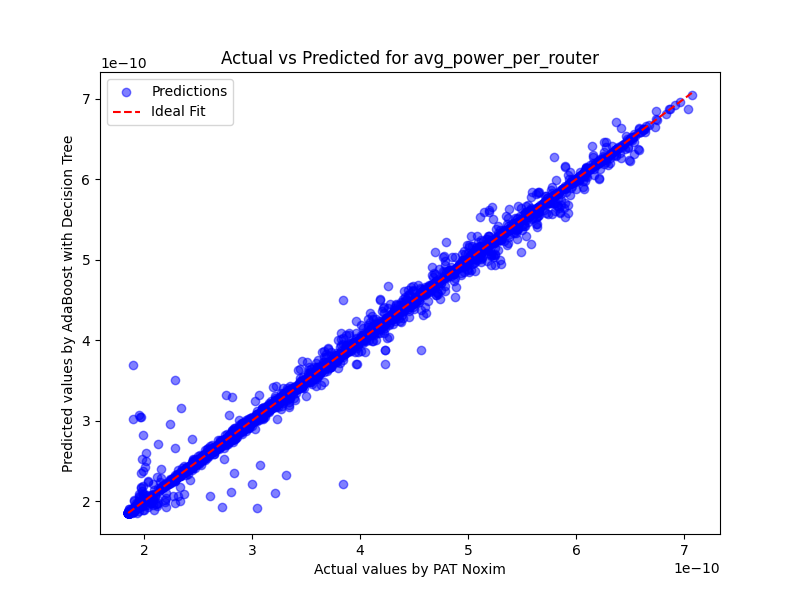
\includegraphics[width=\linewidth]{actual_vs_predicted_avg_power_per_router.png}
        \caption{Actual vs Predicted for avg\_power\_per\_router}
        \label{fig:actual_vs_predicted_avg_power_per_router}
    \end{subfigure}
    \hfill
    % Second graph
    \begin{subfigure}{0.24\textwidth}
        \centering
        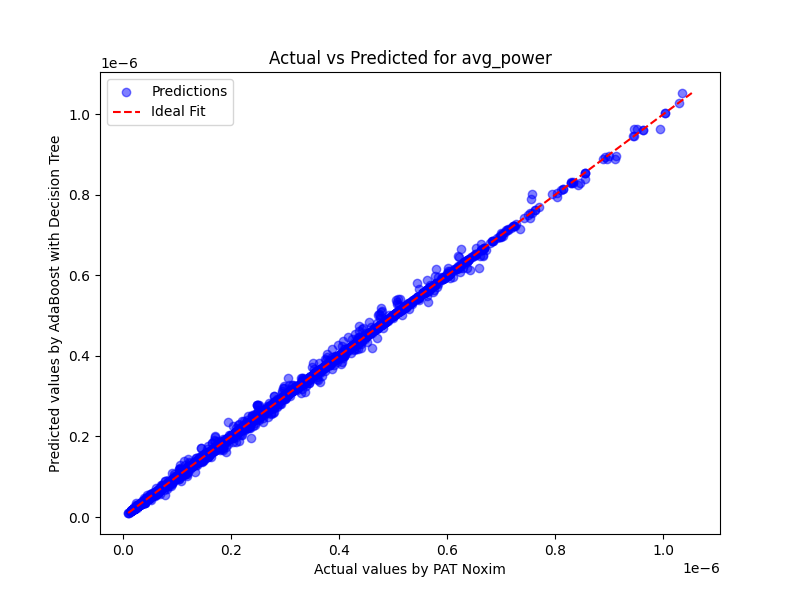
\includegraphics[width=\linewidth]{actual_vs_predicted_avg_power.png}
        \caption{Actual vs Predicted for avg\_power}
        \label{fig:actual_vs_predicted_avg_power}
    \end{subfigure}

    \caption{Actual vs Predicted for avg\_power\_per\_router and avg\_power}
    \label{fig:side_by_side_graphs_avg_power_per_router_avg_power}
\end{figure}

\begin{figure}[htbp]
    % First graph
    \begin{subfigure}{0.24\textwidth}
        \centering
        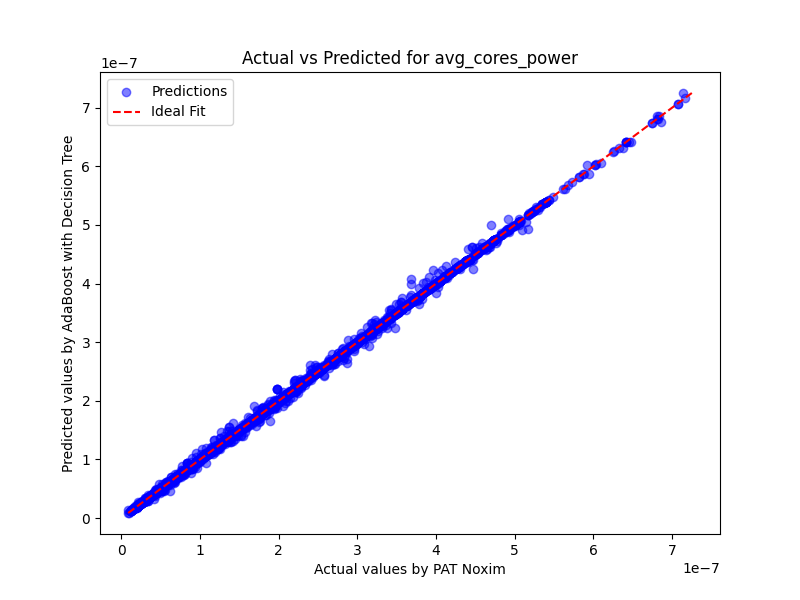
\includegraphics[width=\linewidth]{actual_vs_predicted_avg_cores_power.png}
        \caption{Actual vs Predicted for avg\_cores\_power}
        \label{fig:actual_vs_predicted_avg_cores_power}
    \end{subfigure}
    \hfill
    % Second graph
    \begin{subfigure}{0.24\textwidth}
        \centering
        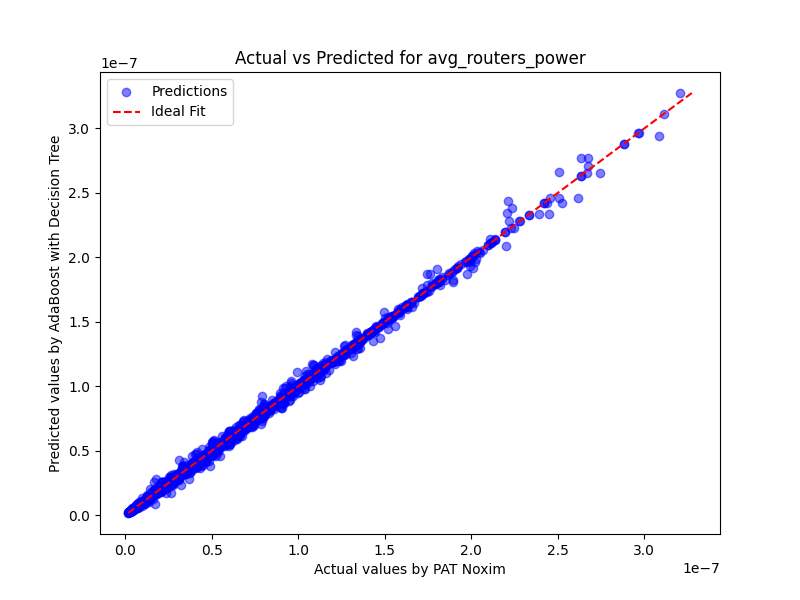
\includegraphics[width=\linewidth]{actual_vs_predicted_avg_routers_power.png}
        \caption{Actual vs Predicted for avg\_routers\_power}
        \label{fig:actual_vs_predicted_avg_routers_power}
    \end{subfigure}

    \caption{Actual vs Predicted for avg\_cores\_power and avg\_routers\_power}
    \label{fig:side_by_side_graphs_avg_cores_power_avg_routers_power}
\end{figure}

\begin{figure}[htbp]
    % First graph
    \begin{subfigure}{0.24\textwidth}
        \centering
        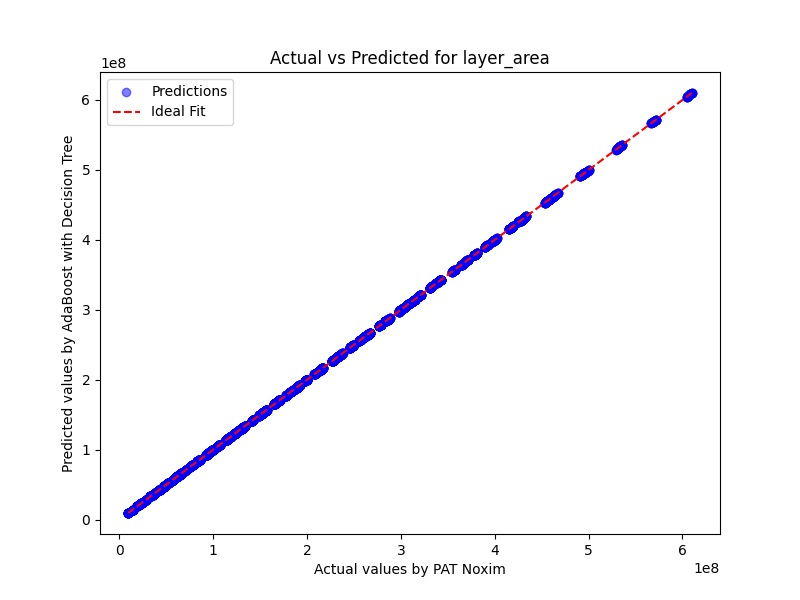
\includegraphics[width=\linewidth]{actual_vs_predicted_layer_area.png}
        \caption{Actual vs Predicted for layer\_area}
        \label{fig:actual_vs_predicted_layer_area}
    \end{subfigure}
    \hfill
    % Second graph
    \begin{subfigure}{0.24\textwidth}
        \centering
        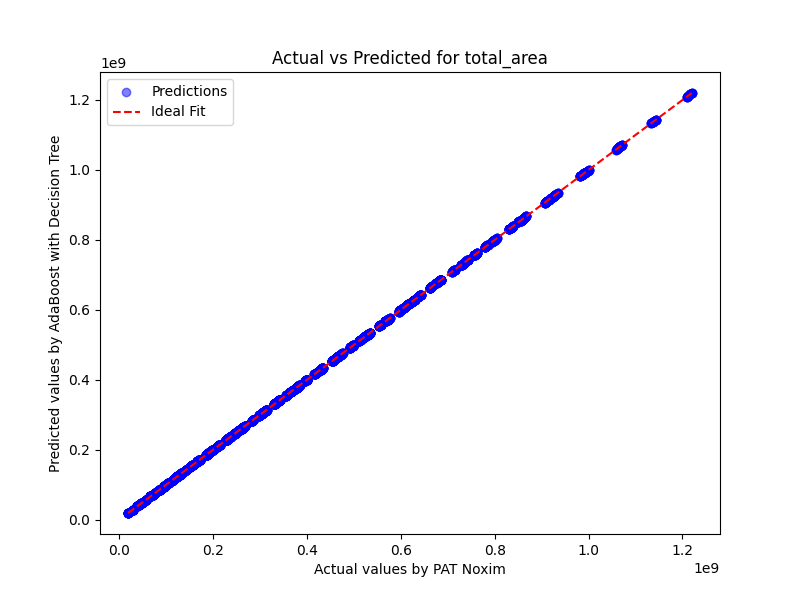
\includegraphics[width=\linewidth]{actual_vs_predicted_total_area.png}
        \caption{Actual vs Predicted for total\_area}
        \label{fig:actual_vs_predicted_total_area}
    \end{subfigure}

    \caption{Actual vs Predicted for layer\_area and total\_area}
    \label{fig:side_by_side_graphs_layer_area_total_area}
\end{figure}

\newpage
\subsection{Execution Time Comparison}
The prediction time of the AdaBoost with Decision Tree model is compared with the simulation time of PAT Noxim simulator for various configurations. The configurations include sqaure mesh sizes ranging from 2 x 2 x 2 to 16 x 16 x 2, pir value of 0.1 and buffer size 8. The routing algorithm are used is XYZ. The simulations are run for 200000 cycles. The traffic considered is Random. The time is recorded in seconds.

\begin{table}[h!]
	\centering
	\begin{tabular}{|c|c|c|}
		\hline
		\textbf{Mesh Size} & \textbf{PAT Noxim (s)} & \textbf{Proposed Method (s)} \\ \hline
		2x2x2              & 13                                      & 0.3359                                     \\ \hline
		3x3x2              & 13                                      & 0.3069                                     \\ \hline
		4x4x2              & 18                                      & 0.4791                                     \\ \hline
		5x5x2              & 26                                      & 0.5367                                     \\ \hline
		6x6x2              & 33                                      & 0.3252                                     \\ \hline
		7x7x2              & 47                                      & 0.5013                                     \\ \hline
		8x8x2              & 78                                      & 0.3649                                     \\ \hline
		9x9x2              & 158                                     & 0.3459                                     \\ \hline
		10x10x2            & 231                                     & 0.1781                                     \\ \hline
		11x11x2            & 318                                     & 0.4136                                     \\ \hline
		12x12x2            & 443                                     & 0.3890                                     \\ \hline
		13x13x2            & 539                                     & 0.3383                                     \\ \hline
		14x14x2            & 673                                     & 0.2346                                     \\ \hline
		15x15x2            & 833                                     & 0.2697                                     \\ \hline
		16x16x2            & 992                                     & 0.4806                                     \\ \hline
	\end{tabular}
	\caption{Simulation time for PAT Noxim and prediction time for the proposed method across different mesh sizes.}
	\label{table:mesh_simulation_time}
\end{table}


It is observed from Table \ref{table:mesh_simulation_time} that the predicted time of the proposed method is much less compared to the simulation time for the PAT Noxim simulator.

\subsection{Scalability}
The PAT Noxim simulator can only simulate a restricted range of mesh sizes up to 16 x 16 x 2. In comparison to the PAT Noxim, the proposed method can predict Power, Area, and Thermal metrics for much larger mesh sizes. The results of predictions for higher configurations are given in Table \ref{tab:higher_config_results}.

\begin{table}[h!]
	\centering
	\begin{tabular}{|l|c|}
		\hline
		\textbf{Parameter} & \textbf{Value} \\ \hline
		Dim X & 32 \\ \hline
		Dim Y & 32 \\ \hline
		Dim Z & 2 \\ \hline
		Buffer Size & 10 \\ \hline
		Packet Size Min & 4 \\ \hline
		Packet Size Max & 8 \\ \hline
		Routing Type & XYZ \\ \hline
		Selection Strategy & Thermal \\ \hline
		Traffic Type & Random \\ \hline
		Injection Rate & 0.05 \\ \hline
		Steady State Temp L0 & 232.220035 \\ \hline
		Steady State Temp L1 & 230.531722 \\ \hline
		Router Avg Temp L0 & 28.161597 \\ \hline
		Router Avg Temp L1 & 27.760194 \\ \hline
		Core Avg Temp L0 & 26.523034 \\ \hline
		Core Avg Temp L1 & 26.333211 \\ \hline
		Mem Avg Temp L0 & 25.952339 \\ \hline
		Mem Avg Temp L1 & 25.828245 \\ \hline
		Total Area & 1.219990e+09 \\ \hline
		Avg Power & 0.000001 \\ \hline
		Avg Cores Power & 7.163280e-07 \\ \hline
		Avg Routers Power & 3.108250e-07 \\ \hline
		Avg Power Per Router & 6.068700e-10 \\ \hline
		Layer Area & 609996000.0 \\ \hline
		Area Per Core & 4695230.0 \\ \hline
	\end{tabular}
	\caption{Higher Configuration Results}
	\label{tab:higher_config_results}
\end{table} 

\subsection{Adaptability}
	
	\subsubsection{Adaptability to routing algorithms}
	The proposed method is capable of predicting for configurations that include different routing algorithms such as XYZ, OE 3D, and Fully Adaptive routing. Tables \ref{table:xyz_routing}, \ref{table:oe_3d_routing}, and \ref{table:fully_adaptive_routing} represent the predicted results of the proposed model and simulation results of PAT Noxim with XYZ, OE 3D, and Fully Adaptive as routing algorithms for the following configurations: Mesh size 8 x 8 x 2, buffer size 10, PIR 0.05, minimum packet size 4, maximum packet size 8, and traffic type random.
	
	% Table for XYZ
	\begin{table}[h!]
		\centering
		\begin{tabular}{|l|c|c|}
			\hline
			\textbf{Parameter} & \textbf{Proposed Method} & \textbf{PAT Noxim} \\ \hline
			Steady State Temp L0 & 167.52312 & 167.580813 \\ \hline
			Steady State Temp L1 & 165.314625 & 165.474859 \\ \hline
			Router Avg Temp L0 & 29.28328 & 29.136848 \\ \hline
			Router Avg Temp L1 & 28.54113 & 28.640883 \\ \hline
			Core Avg Temp L0 & 26.31282 & 26.962495 \\ \hline
			Core Avg Temp L1 & 26.722428 & 26.726645 \\ \hline
			Mem Avg Temp L0 & 26.003424 & 26.008092 \\ \hline
			Mem Avg Temp L1 & 25.829043 & 25.879767 \\ \hline
			Total Area & 304998007.0 & 304998000.0 \\ \hline
			Avg Power & 3.073441e-07 & 3.073450e-07 \\ \hline
			Avg Cores Power & 2.224900e-07 & 2.226330e-07 \\ \hline
			Avg Routers Power & 8.526341e-08 & 8.526710e-08 \\ \hline
			Avg Power Per Router & 6.642208e-10 & 6.661490e-10 \\ \hline
			Layer Area & 152499008.0 & 152499000.0 \\ \hline
			Area Per Core & 4695232.0 & 4695230.0 \\ \hline
		\end{tabular}
		\caption{XYZ Routing}
		\label{table:xyz_routing}
	\end{table}
	
	% Table for OE 3D
	\begin{table}[h!]
		\centering
		\begin{tabular}{|l|c|c|}
			\hline
			\textbf{Parameter} & \textbf{Proposed Method} & \textbf{PAT Noxim} \\ \hline
			Steady State Temp L0 & 124.226720 & 124.186594 \\ \hline
			Steady State Temp L1 & 122.921661 & 122.930750 \\ \hline
			Router Avg Temp L0 & 26.889723 & 26.989448 \\ \hline
			Router Avg Temp L1 & 26.749092 & 26.759092 \\ \hline
			Core Avg Temp L0 &26.285304 & 26.195203 \\ \hline
			Core Avg Temp L1 & 26.167939 & 26.057848 \\ \hline
			Mem Avg Temp L0 & 25.603184 & 25.795822 \\ \hline
			Mem Avg Temp L1 & 25.537649 & 25.700916 \\ \hline
			Total Area & 304998022.0 & 304998000.0 \\ \hline
			Avg Power & 2.162493e-07 & 2.051910e-07 \\ \hline
			Avg Cores Power & 1.620381e-07 & 1.615370e-07 \\ \hline
			Avg Routers Power & 4.142836e-08 & 4.365420e-08 \\ \hline
			Avg Power Per Router & 3.587904e-10 & 3.410490e-10 \\ \hline
			Layer Area & 152499010.0 & 152499000.0 \\ \hline
			Area Per Core & 4695230.0 & 4695230.0 \\ \hline
		\end{tabular}
		\caption{OE 3D Routing}
		\label{table:oe_3d_routing}
	\end{table}
	
	% Table for Fully Adaptive
	\begin{table}[h!]
		\centering
		\begin{tabular}{|l|c|c|}
			\hline
			\textbf{Parameter} & \textbf{Proposed Method} & \textbf{PAT Noxim} \\ \hline
			Steady State Temp L0 & 105.050241 & 105.053375 \\ \hline
			Steady State Temp L1 & 104.175320 & 104.180359 \\ \hline
			Router Avg Temp L0 &26.169781 & 26.174891 \\ \hline
			Router Avg Temp L1 & 26.031640 & 26.033525 \\ \hline
			Core Avg Temp L0 & 25.918263 & 25.92038 \\ \hline
			Core Avg Temp L1 &25.439359 & 25.812806 \\ \hline
			Mem Avg Temp L0 & 25.939359 & 25.739359 \\ \hline
			Mem Avg Temp L1 &  25.841266 & 25.651266 \\ \hline
			Total Area & 304998030.0 & 304998000.0 \\ \hline
			Avg Power &1.482635e-07 & 1.602880e-07 \\ \hline
			Avg Cores Power & 1.508920e-07 & 1.348900e-07 \\ \hline
			Avg Routers Power &2.474189e-08 & 2.538780e-08 \\ \hline
			Avg Power Per Router & 1.920483e-10 & 1.983420e-10 \\ \hline
			Layer Area & 152499010.0 & 152499000.0 \\ \hline
			Area Per Core & 4695230.0 & 4695230.0 \\ \hline
		\end{tabular}
		\caption{Fully Adaptive Routing}
		\label{table:fully_adaptive_routing}
	\end{table}
	
	\subsubsection{Adaptability to 2D}
	The proposed method is capable of predicting Power, Area, and Thermal metrics for 2D mesh sizes as shown in Table \ref{tab:2d_results}.
	
	\begin{table}[h!]
		\centering		
		\begin{tabular}{|l|c|}
			\hline
			\textbf{Parameter} & \textbf{Value} \\ \hline
			Dim X & 4 \\ \hline
			Dim Y & 4 \\ \hline
			Dim Z & 1 \\ \hline
			Buffer Size & 10 \\ \hline
			Packet Size Min & 4 \\ \hline
			Packet Size Max & 8 \\ \hline
			Routing Type & XYZ \\ \hline
			Selection Strategy & Thermal \\ \hline
			Traffic Type & Random \\ \hline
			Injection Rate & 0.05 \\ \hline
			Steady State Temp L0 & 99.3473 \\ \hline
			Router Avg Temp L0 & 27.754863 \\ \hline
			Core Avg Temp L0 & 26.844844 \\ \hline
			Mem Avg Temp L0 & 25.852469 \\ \hline
			Total Area & 76249500.0 \\ \hline
			Avg Power & 7.773150e-08 \\ \hline
			Avg Cores Power & 6.081240e-08 \\ \hline
			Avg Routers Power & 1.691910e-08 \\ \hline
			Avg Power Per Router & 5.287230e-10 \\ \hline
			Layer Area & 38124800.0 \\ \hline
			Area Per Core & 4695230.0 \\ \hline
		\end{tabular}
		\caption{Results for 2D mesh size}
		\label{tab:2d_results}
	\end{table}

\end{document}